\tikzset{every picture/.style={line width=0.75pt}} %set default line width to 0.75pt        

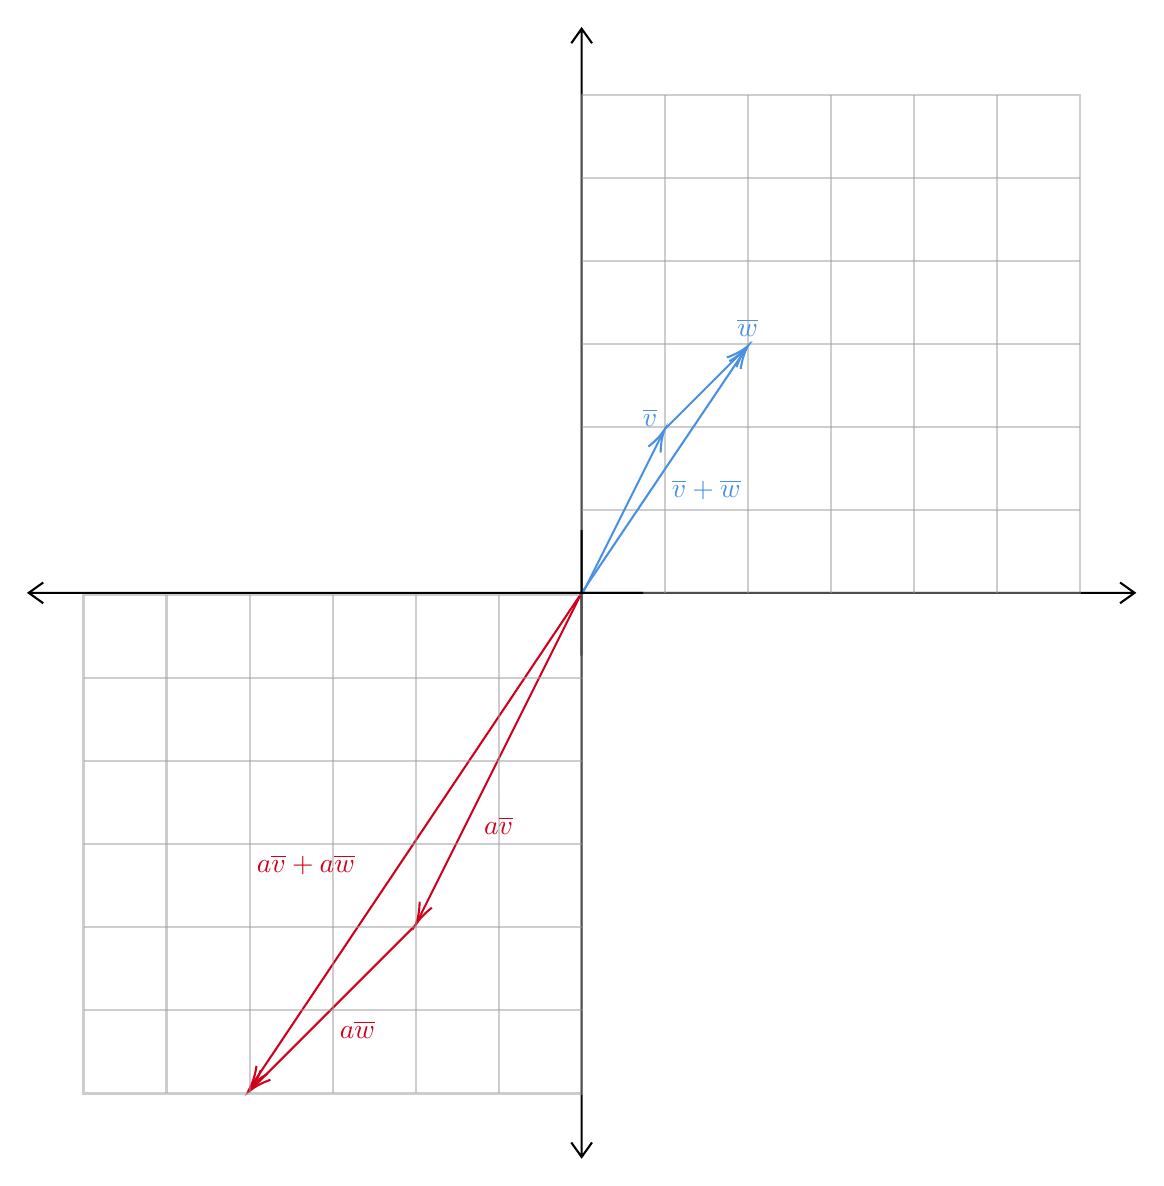
\begin{tikzpicture}[x=0.75pt,y=0.75pt,yscale=-1,xscale=1]
%uncomment if require: \path (0,682); %set diagram left start at 0, and has height of 682

%Shape: Boxed Line [id:dp772165313436463] 
\draw [color={rgb, 255:red, 208; green, 2; blue, 27 }  ,draw opacity=1 ]   (348.6,277.8) -- (189.71,514.94) ;
\draw [shift={(188.6,516.6)}, rotate = 303.82] [color={rgb, 255:red, 208; green, 2; blue, 27 }  ,draw opacity=1 ][line width=0.75]    (10.93,-3.29) .. controls (6.95,-1.4) and (3.31,-0.3) .. (0,0) .. controls (3.31,0.3) and (6.95,1.4) .. (10.93,3.29)   ;
%Shape: Axis 2D [id:dp7962121836036462] 
\draw  (319,277.8) -- (615,277.8)(348.6,6) -- (348.6,308) (608,272.8) -- (615,277.8) -- (608,282.8) (343.6,13) -- (348.6,6) -- (353.6,13)  ;
%Shape: Grid [id:dp7870996256892415] 
\draw  [draw opacity=0] (348.6,37.8) -- (588.6,37.8) -- (588.6,277.8) -- (348.6,277.8) -- cycle ; \draw  [color={rgb, 255:red, 155; green, 155; blue, 155 }  ,draw opacity=0.5 ] (388.6,37.8) -- (388.6,277.8)(428.6,37.8) -- (428.6,277.8)(468.6,37.8) -- (468.6,277.8)(508.6,37.8) -- (508.6,277.8)(548.6,37.8) -- (548.6,277.8) ; \draw  [color={rgb, 255:red, 155; green, 155; blue, 155 }  ,draw opacity=0.5 ] (348.6,77.8) -- (588.6,77.8)(348.6,117.8) -- (588.6,117.8)(348.6,157.8) -- (588.6,157.8)(348.6,197.8) -- (588.6,197.8)(348.6,237.8) -- (588.6,237.8) ; \draw  [color={rgb, 255:red, 155; green, 155; blue, 155 }  ,draw opacity=0.5 ] (348.6,37.8) -- (588.6,37.8) -- (588.6,277.8) -- (348.6,277.8) -- cycle ;
%Straight Lines [id:da6128088926831519] 
\draw [color={rgb, 255:red, 74; green, 144; blue, 226 }  ,draw opacity=1 ]   (388.6,199) -- (427.19,160.41) ;
\draw [shift={(428.6,159)}, rotate = 135] [color={rgb, 255:red, 74; green, 144; blue, 226 }  ,draw opacity=1 ][line width=0.75]    (10.93,-3.29) .. controls (6.95,-1.4) and (3.31,-0.3) .. (0,0) .. controls (3.31,0.3) and (6.95,1.4) .. (10.93,3.29)   ;
%Straight Lines [id:da9944692355606897] 
\draw [color={rgb, 255:red, 74; green, 144; blue, 226 }  ,draw opacity=1 ]   (348.6,277.8) -- (427.48,160.66) ;
\draw [shift={(428.6,159)}, rotate = 123.96] [color={rgb, 255:red, 74; green, 144; blue, 226 }  ,draw opacity=1 ][line width=0.75]    (10.93,-3.29) .. controls (6.95,-1.4) and (3.31,-0.3) .. (0,0) .. controls (3.31,0.3) and (6.95,1.4) .. (10.93,3.29)   ;
%Shape: Boxed Line [id:dp44738419783976924] 
\draw [color={rgb, 255:red, 208; green, 2; blue, 27 }  ,draw opacity=1 ]   (348.6,277.8) -- (269.49,436.01) ;
\draw [shift={(268.6,437.8)}, rotate = 296.57] [color={rgb, 255:red, 208; green, 2; blue, 27 }  ,draw opacity=1 ][line width=0.75]    (10.93,-3.29) .. controls (6.95,-1.4) and (3.31,-0.3) .. (0,0) .. controls (3.31,0.3) and (6.95,1.4) .. (10.93,3.29)   ;
%Straight Lines [id:da27745396609468553] 
\draw [color={rgb, 255:red, 74; green, 144; blue, 226 }  ,draw opacity=1 ]   (348.6,279) -- (387.71,200.79) ;
\draw [shift={(388.6,199)}, rotate = 116.57] [color={rgb, 255:red, 74; green, 144; blue, 226 }  ,draw opacity=1 ][line width=0.75]    (10.93,-3.29) .. controls (6.95,-1.4) and (3.31,-0.3) .. (0,0) .. controls (3.31,0.3) and (6.95,1.4) .. (10.93,3.29)   ;
%Shape: Boxed Line [id:dp5722244470943598] 
\draw [color={rgb, 255:red, 208; green, 2; blue, 27 }  ,draw opacity=1 ]   (268.6,437.8) -- (190.01,516.39) ;
\draw [shift={(188.6,517.8)}, rotate = 315] [color={rgb, 255:red, 208; green, 2; blue, 27 }  ,draw opacity=1 ][line width=0.75]    (10.93,-3.29) .. controls (6.95,-1.4) and (3.31,-0.3) .. (0,0) .. controls (3.31,0.3) and (6.95,1.4) .. (10.93,3.29)   ;
%Shape: Axis 2D [id:dp9489292928363844] 
\draw  (378.2,277.8) -- (82.2,277.8)(348.6,549.6) -- (348.6,247.6) (89.2,282.8) -- (82.2,277.8) -- (89.2,272.8) (353.6,542.6) -- (348.6,549.6) -- (343.6,542.6)  ;
%Shape: Grid [id:dp458334780755161] 
\draw  [draw opacity=0] (348.6,519) -- (108.6,519) -- (108.6,279) -- (348.6,279) -- cycle ; \draw  [color={rgb, 255:red, 155; green, 155; blue, 155 }  ,draw opacity=0.5 ] (308.6,519) -- (308.6,279)(268.6,519) -- (268.6,279)(228.6,519) -- (228.6,279)(188.6,519) -- (188.6,279)(148.6,519) -- (148.6,279) ; \draw  [color={rgb, 255:red, 155; green, 155; blue, 155 }  ,draw opacity=0.5 ] (348.6,479) -- (108.6,479)(348.6,439) -- (108.6,439)(348.6,399) -- (108.6,399)(348.6,359) -- (108.6,359)(348.6,319) -- (108.6,319) ; \draw  [color={rgb, 255:red, 155; green, 155; blue, 155 }  ,draw opacity=0.5 ] (348.6,519) -- (108.6,519) -- (108.6,279) -- (348.6,279) -- cycle ;

% Text Node
\draw (386.6,199.1) node [anchor=south east] [inner sep=0.75pt]  [color={rgb, 255:red, 74; green, 144; blue, 226 }  ,opacity=1 ]  {$\overline{v}$};
% Text Node
\draw (428.6,155.6) node [anchor=south] [inner sep=0.75pt]  [color={rgb, 255:red, 74; green, 144; blue, 226 }  ,opacity=1 ]  {$\overline{w}$};
% Text Node
\draw (390.6,221.8) node [anchor=north west][inner sep=0.75pt]  [color={rgb, 255:red, 74; green, 144; blue, 226 }  ,opacity=1 ]  {$\overline{v} +\overline{w}$};
% Text Node
\draw (308.6,395.6) node [anchor=south] [inner sep=0.75pt]  [color={rgb, 255:red, 208; green, 2; blue, 27 }  ,opacity=1 ]  {$a\overline{v}$};
% Text Node
\draw (230.6,482.4) node [anchor=north west][inner sep=0.75pt]  [color={rgb, 255:red, 208; green, 2; blue, 27 }  ,opacity=1 ]  {$a\overline{w}$};
% Text Node
\draw (190.6,402.4) node [anchor=north west][inner sep=0.75pt]  [color={rgb, 255:red, 208; green, 2; blue, 27 }  ,opacity=1 ]  {$a\overline{v} +a\overline{w}$};


\end{tikzpicture}
